\begin{Problem}
	\begin{parts}
	\item Skizzieren Sie die Menge
		\[
		Q=\{w\in \C:|\Re w|+|\Im w|=1\} 
		.\] 
	\item Es sei $g:\R \to \R,~g(x)=|x|$. Zeigen Sie, dass $g$ in $x_0\in \R\setminus \{0\} $ differenzierbar ist und bestimmen Sie $g'(x_0)$.
	\item Es sei $G$ ein Gebiet in $\C$, $f:G\to \C$ holomorph, $u:=\Re f$ und $v:=\Im f$. Zeigen Sie: Falls $|u(z)|+|v(z)|=1$ f\"{u}r jedes $z\in G$, so ist $f$ konstant auf $G$.
	\end{parts}
\end{Problem}

\begin{proof}
	\begin{parts}
	\item \noindent \\ 
		\begin{center}
		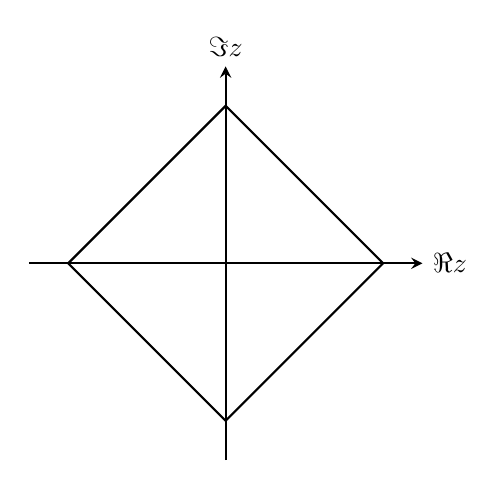
\begin{tikzpicture}[scale=2.5]
			\draw[thick, -stealth] (-1,0) -- (1,0) node[anchor=west] {$\Re z$};
			\draw[thick, -stealth] (0,-1) -- (0,1) node[anchor=south] {$\Im z$};
			\draw[thick] (0.8,0) -- (0,0.8) -- (-0.8,0) -- (0,-0.8) -- cycle;
		\end{tikzpicture}
	\end{center}
\item F\"{u}r $x_0\in \R\setminus \{0\} $ gibt es eine Umgebung $U$ um $x_0$, so dass entweder $g(x)=x$ oder $g(x)=-x$ gilt. Daher ist der Grenzwert, durch den die Ableitung definiert ist, immer gleich der Grenzwert mit $x$ oder $-x$. Die Ableitung ist also
	\[
	g'(x_0)=\begin{cases}
		1 & x_0 > 0,\\
		-1 & x_0 < 0.
	\end{cases}
	\] 
\item Das Bild in (a) enthält 4 Geraden. Wir betrachten zwei Fälle
	\begin{enumerate}[label=(\roman*)]
		\item $f(G)$ enthält keine der Ecken

			In diesem Fall ist $f(G)$ eine Teilmenge einer Strecke. Durch Verkettung mit einer linearen Funktion $g(x)$ können wir das Bild als Teilmenge der reellen Achse betrachten, $g(f(G))\subseteq \R$. $f$ ist genau dann holomorph, wenn $g\circ f$ holomorph ist.

			Aber $g\circ f$ muss dann konstant sein.

			\begin{Lemma}
				Holomorphe funktionen $h:\C\to \R$ sind konstant.
			\end{Lemma}
			\begin{proof}
				\begin{align*}
					h'(z_0)=&\left.\pdv{h}{x}\right|_{z_0}\\
					=&\lim_{x \to x_0} \frac{h(x+iy_0)-h(x_0+iy_0)}{x-x_0}\in \R\\
					h'(z_0)=&\left. \pdv{h}{y}\right|_{z_0}\\
					=&\lim_{y \to y_0} \frac{h(x+iy)-h(x+iy_0)}{iy-iy_0} \in \{0\} \times \R\subseteq \C
				\end{align*}
				Das heißt: $h'(z_0)=0$ f\"{u}r alle $z_0\in \C$ und $h$ ist konstant.
			\end{proof}
		\item $f(G)$ enthält mindestens eine der Ecken

			Sei $z_0$, sodass $f(z_0)$ die Ecke ist. Wir zeigen: $f$ ist nicht im $z_0$ differenzierbar. Es gibt eine stetig differenzierbare Kurve $\gamma:(\alpha,\beta)\to \C$, so dass $z_0\in \gamma( (\alpha,\beta))$. Dann ist $f(\gamma(t))$ nicht differenzierbar, ein Widerspruch, weil $f$ holomorph ist und deswegen $\dv{t}(f(\gamma(t)))=f'(\gamma(t))\gamma'(t)$ gelten soll.\qedhere
	\end{enumerate}
	\end{parts}
\end{proof}

\begin{Problem}
	\begin{parts}
	\item Es sei
		\[
		g:\C\setminus \{-1\} \to \R, \qquad g(x)=\log\left( \frac{1}{|1+z|^2} \right)
		.\] 
		Zeigen Sie, dass $f:\mathbb{D}\to \C,~f(z)=\pdv{g}{z}(z)$ eine auf $\mathbb{D}$ holomorphe Funktion definiert.
	\item Es sei
		\[
		g:\C\to \R,\qquad g(z)=\log\left( \frac{1}{1+|z|^2} \right)
		.\] 
		Definiert auch in diesem Fall $f:\mathbb{D}\to \C,~f(z)=\pdv{g}{z}(z)$ eine auf $\mathbb{D}$ holomorphe Funktion?
	\end{parts}
\end{Problem}
\begin{proof}
	\begin{parts}
	\item Definiere $z=x+iy$, also
	\begin{align*}
		|1+z|^2=&|1+x+iy|^2\\
		=&(1+x)^2 + y^2
	\end{align*}
	Die partielle Ableitungen sind
	\begin{align*}
		\pdv{g}{x}=&\pdv{x} \log\left( \frac{1}{(1+x)^2+y^2} \right)\\
		=& ( (1+x)^2+y^2) \pdv{x} \frac{1}{(1+x)^2+y^2}\\
		=& -\frac{2(1+x)}{(1+x)^2+y^2}\\
		\pdv{g}{y}=&-\frac{2y}{(1+x)^2+y^2}\\
		\pdv{g}{x}=& \frac{1}{2}\left( \pdv{g}{x}-i\pdv{g}{y} \right)\\
		=&-\left[\frac{1+x}{(1+x)^2+y^2}-\frac{iy}{(1+x)^2+y^2} \right]\\
		=&- \frac{1+x-iy}{1+2x+x^2+y^2}\\
		=&- \frac{1+x-iy}{(1+x+iy)(1+x-iy)}\\
		=&-\frac{1}{1+x+iy}\\
		=&- \frac{1}{1+z}
	\end{align*}
	was offensichtlich holomorph ist.
\item Wie üblich $z=x+iy$ und damit $1+|z|^2=1+x^2+y^2$. Die partielle Ableitungen sind
	\begin{align*}
	g(x,y)=& \log\left( \frac{1}{1+x^2+y^2} \right)\\
	\pdv{g}{x}=&-\frac{2 x}{x^2+y^2+1}\\
	\pdv{g}{y}=&-\frac{2 y}{x^2+y^2+1}\\
	\pdv{g}{z}=&-\left( \frac{x}{x^2+y^2+1}-i\frac{y}{x^2+y^2+1} \right)\\
	f(x,y)=&-\frac{x-iy}{1+x^2+y^2}
	\end{align*}
	Die partielle Ableitungen von $f$ sind
	\begin{align*}
		\pdv{f}{x}=&\frac{-x^2+2 i x y+y^2+1}{\left(x^2+y^2+1\right)^2}\\
		\pdv{f}{y}=&-\frac{i \left(x^2-2 i x y-y^2+1\right)}{\left(x^2+y^2+1\right)^2} 
	\end{align*}
	Die Cauchy-Riemannsche Differentialgleichung
	\[
	\pdv{f}{x}=-i\pdv{f}{y}
	\]
	gilt nicht, also $f$ ist nicht holomorph.\qedhere
\end{parts}
\end{proof}

\begin{Problem}
	Gegeben sei $a\in \mathbb{D}$ und die Möbiustransformation
	\[
	T_a:\mathbb{D}\to\mathbb{D},\qquad T_a(z)=\frac{a+z}{1+\overline{a}z}
	.\] 
	Ferner bezeichne $\mathbb{D}^+:=\{z\in \mathbb{D}:\Im z>0\} $ die obere Einheitskreisscheibe. Zeigen Sie, dass $T_a(\mathbb{D}^+)\subseteq \mathbb{D}^+$ genau dann gilt, wenn $\Im a\ge 0$.
\end{Problem}

\begin{proof}
	``$\implies$''

	Wir beweisen: Wenn $\Im a<0$, ist $T_a(\mathbb{D}^+)\not\subseteq \mathbb{D}^+$. Wenn $\Im a<0$, ist $-a\in \mathbb{D}^+$. Damit gilt
	\[
	T_a(-a)=0\not\in \mathbb{D}^+
	.\] 
	
	Jetzt $\impliedby$. Die Umkehrabbildung ist
\[
T_a^{-1}(z)=\frac{z-a}{1-\overline{a}z}
.\] 
	Wir betrachten das Bild des Rands. Zuerst betrachten wir das Bild von $[-1,1]\times \{0\} \subseteq \C$.
\begin{align*}
	T_a(0)=& a\in \overline{\mathbb{D}^+}\\
	T_a(1)=&\frac{1+a}{1+\overline{a}}\\
	|T_a(1)|=& 1 & \text{siehe \eqref{eq:complexanal3-1}}\\
	\angle T_a(1)=&\angle (1+a) - \angle (1+\overline{a})\\
	=&2\tan^{-1}\left( \frac{\Im a}{\Re a+1} \right)\\
	\ge& 0 & \Im a > 0\\
	T_a(-1)=&\frac{a-1}{1-\overline{a}}\\
	|T_a(-1)|=&1 & \text{siehe \eqref{eq:complexanal3-1}}\\
	\angle T_a(-1)=& \angle (a-1) - \angle (1-\overline{a})\\
	=& 2\tan^{-1}\left( \frac{\Im a}{\Re a - 1} \right)\\
	\ge& 0
\end{align*}
Nebenrechnung: 
\begin{align*}
	|1+a|=&(1+a)(1+\overline{a})\\
	=&1+a+\overline{a}+|a|^2\\
	=&1+2\Re a+|a|^2\\
	=&1 + 2\Re \overline{a}+|\overline{a}|^2\\
	=&|1+\overline{a}|\addtocounter{equation}{1}\tag{\theequation}\label{eq:complexanal3-1} 
\end{align*}
Daher sind $T_a(0),~T_a(1)$ und $T_a(-1)$ alle Elemente von $\mathbb{D}^+$. Jetzt betrachten wir
\begin{align*}
	T_a(i)=&\frac{a+i}{1-i\overline{a}}\\
	|T_a(i)|=& 1 & \text{auch ähnlich wie \eqref{eq:complexanal3-1}}
\end{align*}
Der Rand $\partial \mathbb{D}^+$ wird auf einer Teilmenge von $\mathbb{D}^+$ abgebildet, also $T_a(\partial\mathbb{D}^+)\subseteq \mathbb{D}^+$. Aus einer ähnliche Rechnung erhalten wir, dass $T_a(-i)\in \C\setminus \overline{\mathbb{D}^+}$. Daher schließen wir, dass die Außenseite des $\overline{\mathbb{D}^+}$ wieder auf die Außenseite des $\overline{\mathbb{D}^+}$ abgebildet wird. Weil $T_a$ bijektiv ist, muss das Innere des $\mathbb{D}^+$ nach $\mathbb{D}^+$ abgebildet werden, also $T_a(\mathbb{D}^+)\subseteq \mathbb{D}^+$.
\end{proof}
